
%--------------- Chapter 1: Introduction ---------------%

\chapter{INTRODUCTION}\label{Ch1:Introduction}
\graphicspath{{Chapter1/Chapter1Figs/}{Chapter1/Chapter1Figs/}}

Image classification process categorizes various images into their corresponding classes. A large number of application areas uses image classification as one of the prime phases such as medical imaging, robotics, computer vision, and many more. However, due to the variations available in the images, a single classification process cannot be used for all the application areas. Out of many applications, medical imaging is of prime importance which directly influences the society and its automation helps for unbiased analysis of various diseases. Histopathological image analysis also is one of the important areas of medical imaging which is generally performed manually by the pathologists. It is a necessary part of  drug development in the pharmaceutical companies and also used by pathologists for disease identification.

Histopathology is the investigation of tissues to identify the symptom of abnormality. This process is generally done by trained pathologists manually in the pathology labs. Generally, tissues are colorless, therefore, various staining methods are used to provide the colors. Among various staining methods, hematoxylin and eosin (H\&E) staining is widely used. It provides a blue color to the nuclei and pink or red color to the cytoplasm. Due to the advancements in digital electronics, pathology labs are going to be transformed into the digital era \cite{stathonikos2013}. The high-quality whole-slide image (WSI) scanners capture the images at very high resolutions from the tissue samples.  Figure \ref{ch1:fig:HI} depicts two sample histopathological images having healthy and inflamed tissues respectively. 
\begin{figure}[h!]
            \begin{center}
            \subfigure[Healthy tissue]{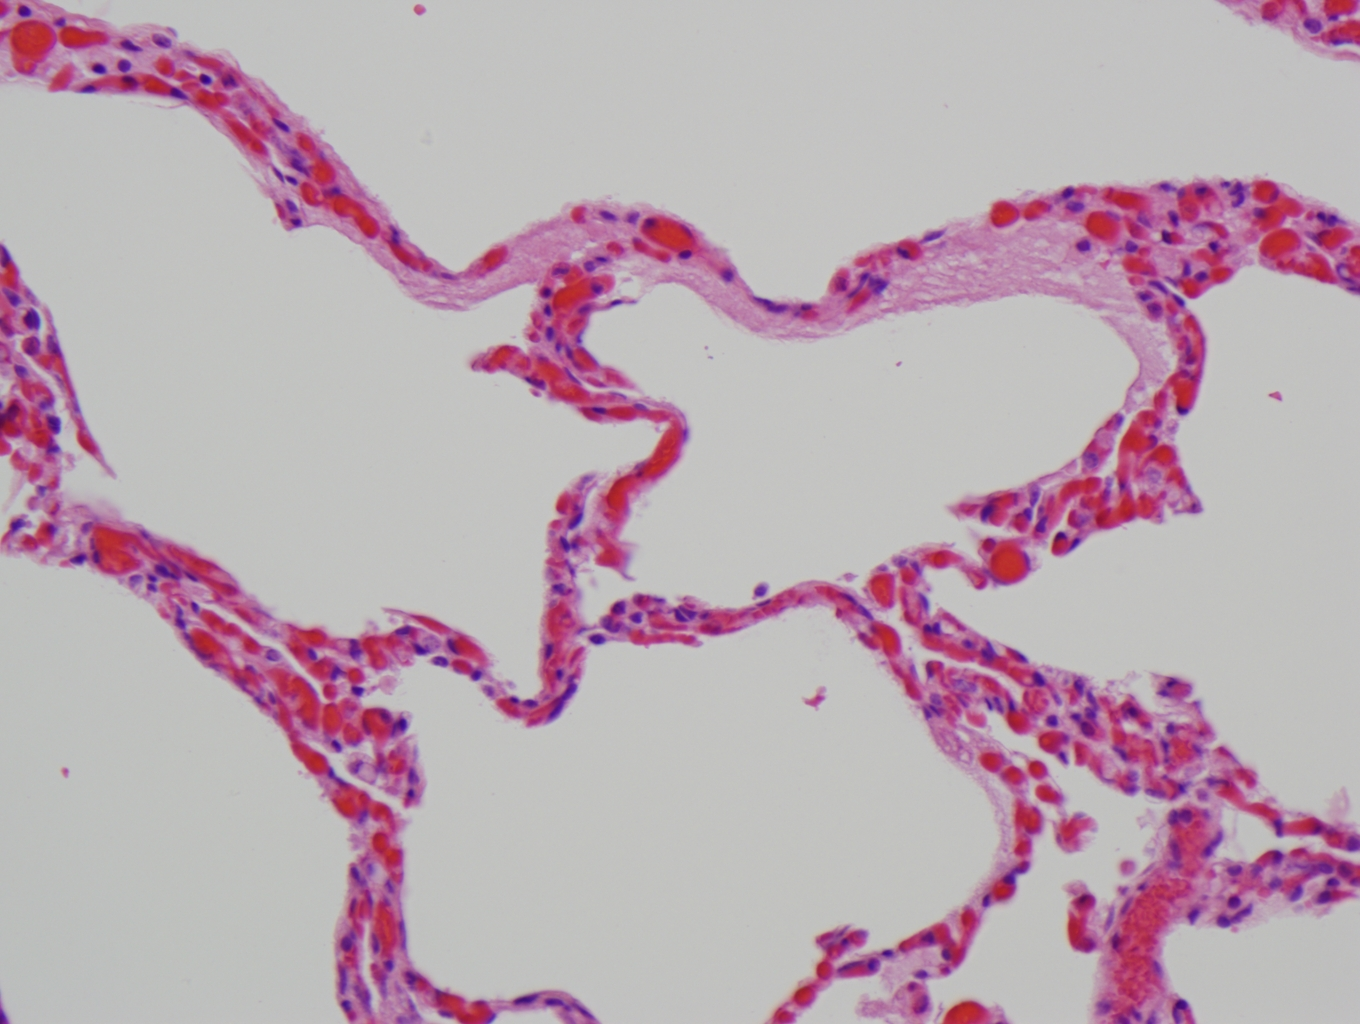
\includegraphics[width=0.4\textwidth]{LN}}~~~~~
        \subfigure[Inflamed tissue]{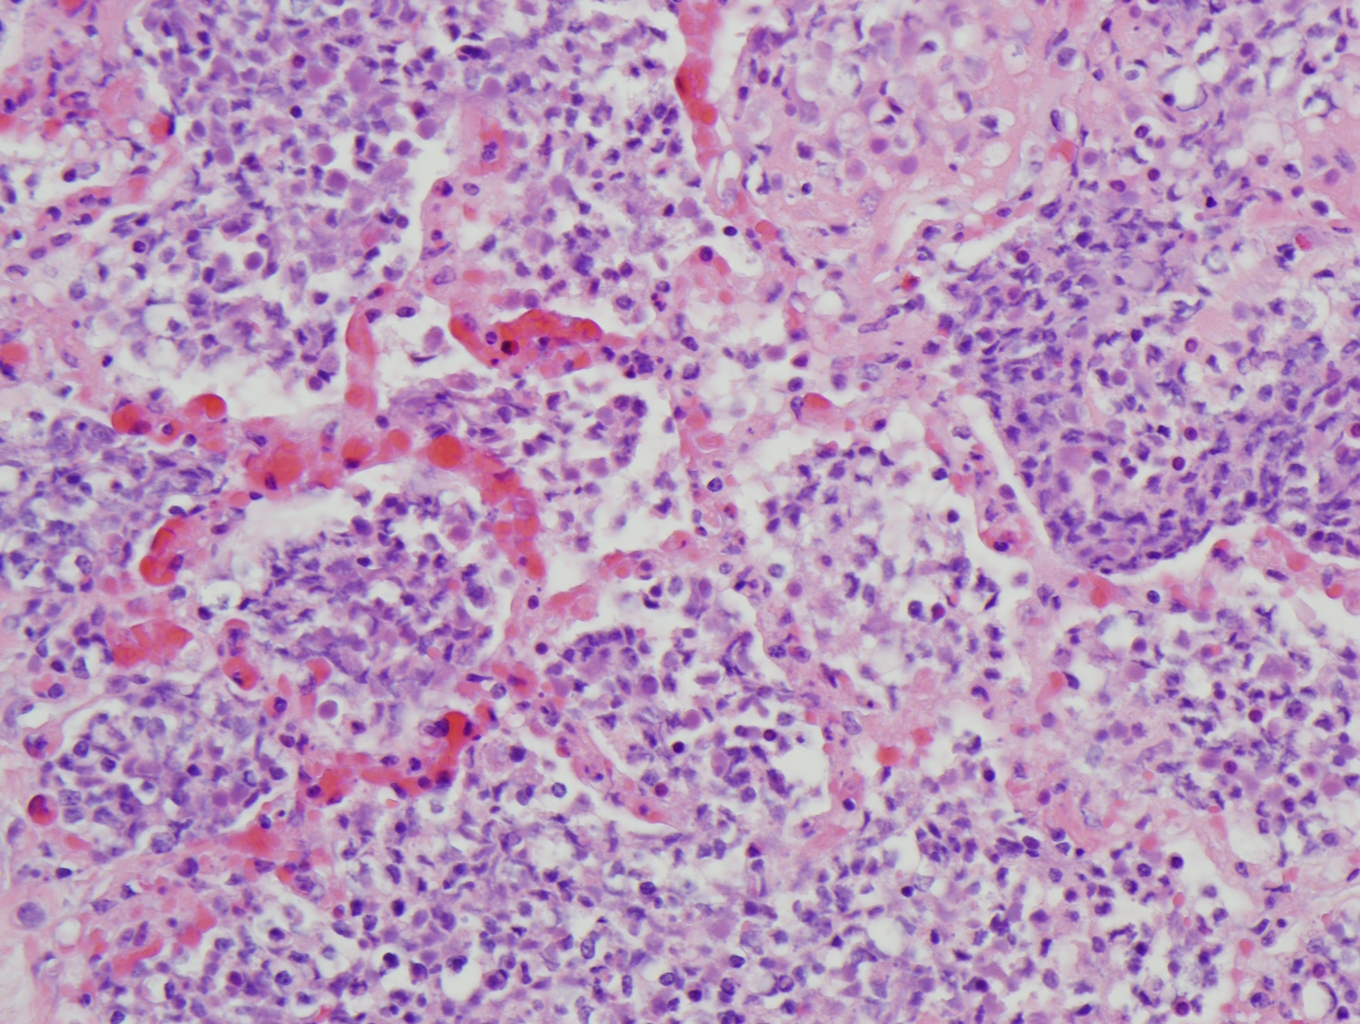
\includegraphics[width=0.4\textwidth]{LI}}
 \end{center}
    \caption[Histopathological images]{Histopathological images \cite{srinivas2014}}
    \label{ch1:fig:HI}
\end{figure}
The digitization of tissue slides has substantially made accurate decisions for disease diagnosis \cite{srinivas2014}. The pathologists can view the tissue images on computer monitors but, still the analysis of the tissue sections is very time taking and biased due to the experience and knowledge of the pathologists. Therefore, there is a requirement to develop an automated method for histopathological image classification. It is a promising area that acquires the attention of the researchers \cite{gurcan2009}. These automated systems help the pathologists in the decision-making process for the diagnosis of the disease \cite{mccann2014}. The improvement of computer technologies and digitization of histopathological images further increase the need for such automated systems for the pathologists. Therefore, this work focuses on the development of significant automated methods for histopathological image classification.

This chapter presents the research motivation followed by a brief introduction to histopathological image analysis, the challenges of histopathological image classification, and the organization of the thesis.

\section{Motivation}\label{ch1:sec:Motivation}
The past decade has shown an exponential increase in computational efficiency along with better image analysis techniques. These have insisted to develop the powerful machine learning algorithms for medical image analysis. Furthermore, the development of whole slide scanners for histopathological tissue slides, the digital histopathological images are used for analyses. However, due to the various variabilities and complexities available in the images, this analysis is performed manually by the expert pathologists. The manual histopathological image analysis is time taken process and  also biased. The report generated by a pathologist is generally dependent on his knowledge and experience. Therefore, the automation of this task helps the pathologists to work efficiently with machine intelligence. Secondly, by automatically identifying the inflamed images, the observer variability can be eliminated and this can also improve the accuracy of disease diagnosis. However, the automation of the classification of histopathological images is a difficult process due to the morphological complexity and technical variations of histopathological images such as different organ types, variations of devices used, the orientation of slides, and different staining methods \cite{basavanhally2009}. 
Moreover, histopathological images contain an enormous density of data as compared to radiological and other imaging modalities. This makes the descriptor design task very complex which affects the performance of an automated image classification system \cite{gurcan2009}.  Therefore, this work aims to develop an improved system to classify histopathological images and  resolve constraints related with existing methods.

\section{Histopathological Images Analysis}


The histopathological image analysis is used in the development of drugs and the identification of the diseases. Regardless of the popularity of modern diagnostic tools in the biomedical field, histopathological image analysis is still performed manually. The manual analysis of these images takes lots of time and efforts of the dedicated pathologists. Some major problems of  manual analysis of these images are enlisted below:

\begin{itemize}
\item \textbf{Scarcity of expert pathologists:} Due to the advancements in medical technology, pathology labs generate a lot of data every year and it is required to handle this data daily by the pathologists. Hence, there is a high demand for expert pathologists all over the world. In Australia, a shortage of pathologists impacts the international workforce as acknowledged by the advisory committee of the Australian Medical Workforce \cite{cancer2010}.


\item \textbf{Variability and biased observations \cite{gurcan2009} \cite{cigdem2005}:} 
The experience and knowledge of different pathologists may vary which impact the opinion given by them for the same histopathological image. These variations may result in wrong treatment and sometimes delayed treatment.


\item \textbf{Complexity and variability in biological structures among tissue slides \cite{gurcan2009}:}
Histopathological images contain various morphological structures and complexities such as the use of different staining dyes, illumination variations at the time of capturing the images, different shapes and sizes of nuclei, and many more. It is very hard for the pathologists to analyze all these variabilities.

\item \textbf{Consumption of time and efforts:}
The manual analysis of a histopathological image requires at least three to four hours of sitting and evaluation of quantitative properties makes it a more complex task. Further, if the images are captured at a high magnification rate then more time is needed by the pathologists to analyze the whole slide.
\end{itemize}

To overcome the shortcomings mentioned above, the automated analysis of histopathological images may be used. An automated image analysis system  can provide meaningful data more accurately and timely for the histopathological images. This reduces the workload on the pathologists and makes less human subjectivity. This process enhances the manual analysis process by generating reliable and fast results. Recent advancements in the computer vision and image analysis open up various opportunities to design and develop an automated image classification system for histopathological images. 
These systems help in making unbiased, efficient, and accurate analysis reports promptly and perform automated classification of different tissue types which can be accessible widely as a tool for research. 

Therefore, the development of automated histopathological image classification methods has emerged as a significant research problem in medical imaging \cite{gurcan2009}\cite{srinivas2014}\cite{saraswat2013}. However, there are many problems associated with the development of such automated system. The following section discusses the various challenges in the automation of histopathological image classification. 



\section{Challenges}\label{ch1:sec:Challenges}
Though many histopathological image classification methods are available in the literature which show quite promising results, still there exists some challenges which affect the accuracy of the system. This needs the attention of the researchers the for improvements so that the expectations of the pathologists can be fulfilled.


\begin{enumerate}
\item \textbf{Variations in the color and illumination:}  Histopathological images are the colorful tissue images after staining and captured by the whole slide scanners. The color provided by staining methods may vary as it is a manual process and similarly, there may be variations in the illumination light while capturing the images. These color and illumination variations may degrade the performance of the automated system significantly \cite{magee2009}.

\item \textbf{Different methods for staining:} 
Most of the works for histopathological image analysis have been done on tissue section images stained with some chemicals like immunohistochemical (IHC), immunofluorescence (IF), and hematoxylin \& eosin (H\&E). These staining procedures are very expensive and time-taking. The use of multiple staining methods for the preparation of histopathological images makes the analysis difficult for the automated methods \cite{gurcan2009} \cite{Ong1996}.

\item 
\textbf{Enormous density of data:}
Another challenge in the automated histopathological image analysis is the huge density of the data as compared to other biomedical images like tomography, radiology, and other image modalities, which has to be contended by the automated methods. For example, the chest CT scan, captured on high resolution, consists of approximately $143$ million pixels with $ 512\times512\times512$ spatial elements. On another hand, the biopsy tissue of the prostate, captured at $40\times$ resolution by a whole slide image scanner, consists of approximately $235$ million pixels with $15,000\times15,000$ elements. Moreover, for one patient study, there is a requirement of $10$ to $20$ biopsy samples which results in generating a huge data of approximately $3$ to $4$ billion pixels. Therefore, unlike the automated methods proposed for radiology and other medical imaging, automated histopathological image analysis methods are usually built in such a way that they have to perform efficiently and accurately on the high density of data.

\item \textbf{Multimodal data fusion:}
Histopathology is generally used to study the cancer disease in the patients but the diagnosis and prognosis of the cancer disease are very hard. If two patients are going through the same treatment procedure with the same disease may result in different outcomes. The reason for this difference may be patient specific or it may be due to the lack of related information between the progression of the disease and clinical aspects. There is a common consent between scientists and pathologists that the understanding of tumor visual morphology using automated image analysis methods along with the disease classification will result in better treatment and patient care. Therefore, multimodal data fusion has emerged as a relevant challenge for digital pathology labs for making the recommendation about the patient treatments. 

\item \textbf{Maintenance of image data:}
Due to the advancements in digital imaginary tools and image acquisition methods, a large amount of data is generated. The storage, registration, maintenance, and transmission of such a big volume of data is a challenging task. The spectral imaging data from the whole slide scanner makes the problem more complex. 

\end{enumerate}

\section{Scope of the Thesis}\label{ch1:sec:Scope of the Thesis}

For histopathology, computer vision, and biomedical scientists, the above-mentioned challenges will open various research problems and opportunities to develop new image analysis methods. The pathologists and computer scientists work together in collaboration with microscopy and slide scanner vendors to build innovative and novel methods to solve various challenges of image analysis in digital pathology. Furthermore, in recent years, there is a rapid increase of histopathological digital images over the Internet and there is a need to organize them properly for better retrieval and analysis processes for the researchers. Therefore, an automated histopathological image classification system can be useful. In literature, several automated histopathological image classification methods exist which are based on the approaches like a graph, hashing, bag-of-features, and deep neural networks. The Bag-of-features method is one of the well-liked image classification methods and shows better performance when applied to histopathological images. However, there is a requirement for improvement in the different phases of the bag-of-features method. The main objective of this thesis is to design and develop an efficient histopathological image classification system based on the bag-of-features method. The main contribution of the thesis is five-fold. It first aims to develop an efficient keypoints selection method to find the relevant and discriminative features from histopathological images. Second, to reduce the effect of the dense region in the codebook construction phase of the bag-of-features method, a meta-heuristic based codebook construction method has been introduced. Third, a new and computationally efficient codebook construction method is designed and developed to find relevant visual words. Fourth, an efficient feature encoding method has to be designed and developed by incorporating the merits of two different features descriptors for the better image representation and finally, an enhanced bag-of-features method is developed by incorporating the newly introduced methods for the classification of histopathological images.  The complete workflow of the thesis is shown in Figure \ref{ch1:fig:The flow chart of the proposed research work}.
\begin{figure}[h]
\centering
     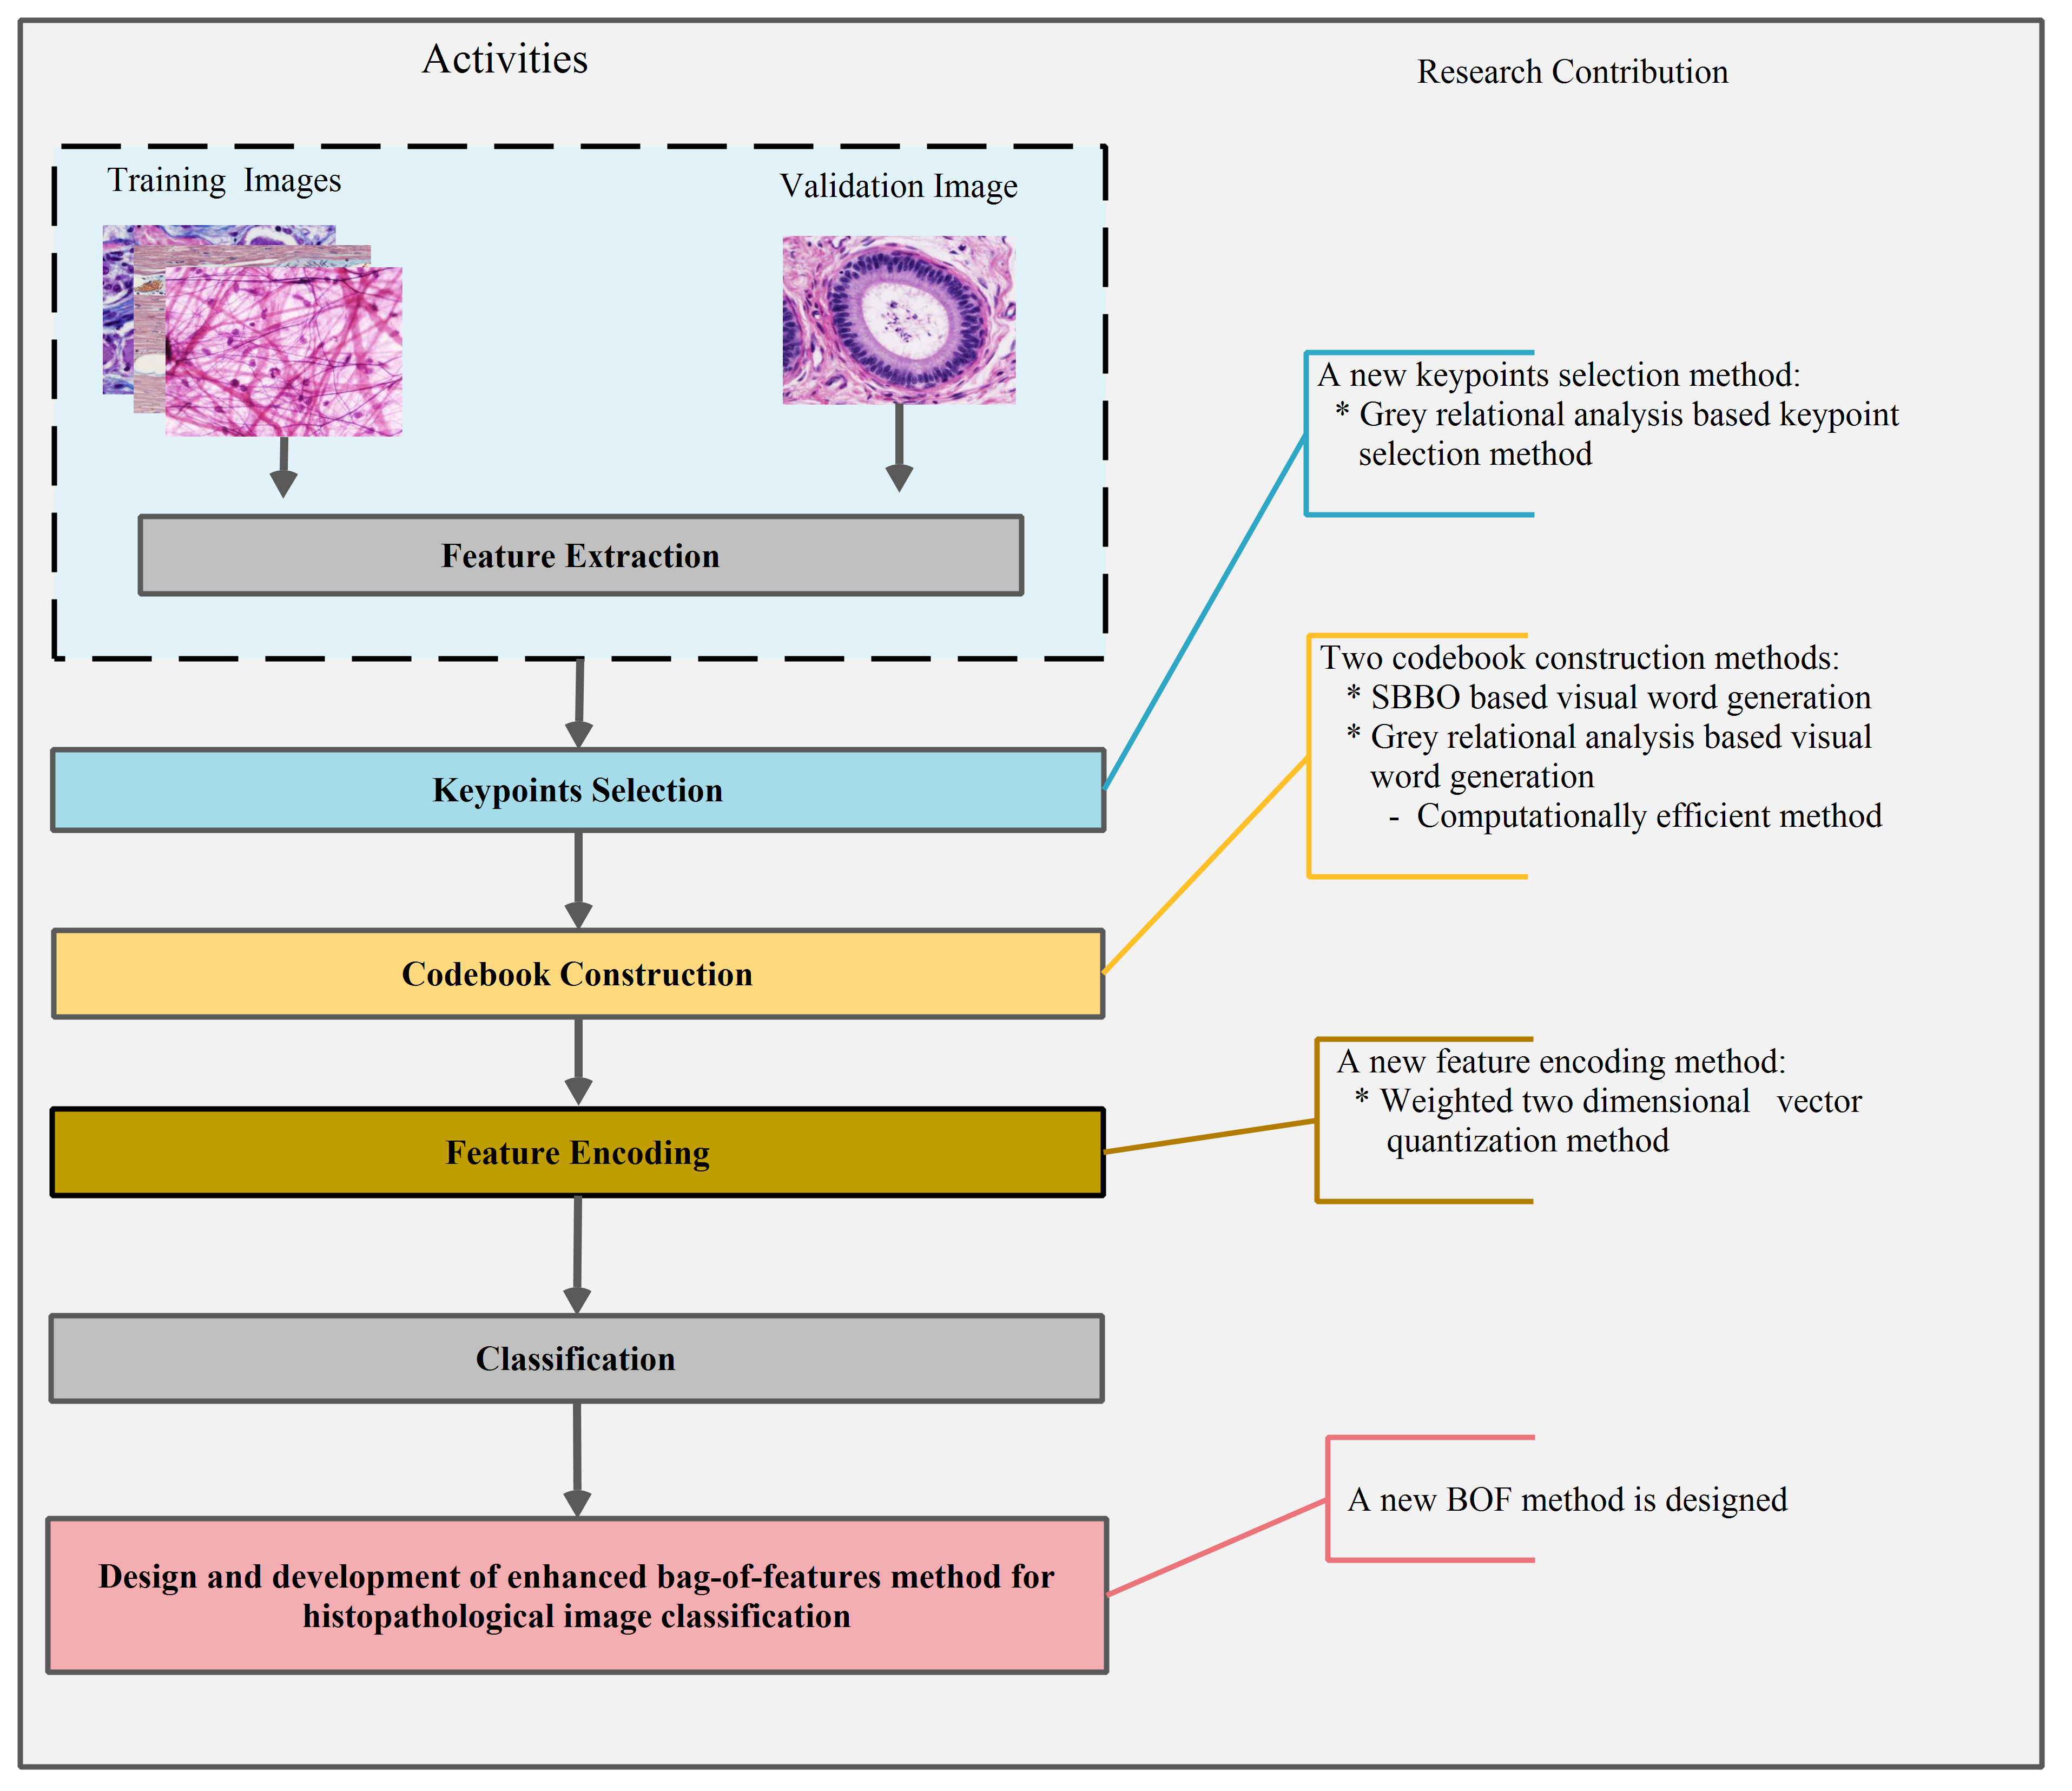
\includegraphics[width=\textwidth]{RM1}
   \caption [The work flow of the proposed research work]{\fontsize{10pt}{12pt}\selectfont The work flow of the proposed research work}
 \label{ch1:fig:The flow chart of the proposed research work}
\end{figure}
The rest of the material is arranged in the following chapters.

\paragraph{Chapter 2} surveys the existing methods for histopathological image classification along with a detailed literature survey presented for the different phases of the bag-of-features method. Based on the outcome of this study, research gaps are identified and documented along with the corresponding research objectives.

\paragraph{Chapter 3} deals with the problem of a large number of keypoints descriptors generated by feature extraction method for histopathological images. This chapter presents a new keypoints selection method based on a grey relation analysis for finding relevant and useful features. The method is introduced before the codebook construction phase of the bag-fo-features method. The new method is validated against other state-of-the-art keypoints selection methods. For a fair comparison, two standard histopathological image datasets are used. 

\paragraph{Chapter 4} studies the biogeography-based optimization, as it has been used effectively to classify the medical images as compared to other nature-inspired methods available in the literature. However, sometimes it shows a slow convergence rate and poor precision due to its single feature migration property and poor mutation. Therefore, this chapter presents two variants of biogeography-based optimization, namely improved biogeography-based optimization and spiral biogeography-based optimization, to mitigate its demerits. With the experimental and statistical analysis over two benchmark sets, the new variants have been compared with recent meta-heuristic methods. The new methods have been used to develop an effective codebook in the bag-of-features methods and reduce the effect of dense regions of histopathological images. The modified bag-of-features method is compared with other state-of-the-art methods over two standard histopathological image datasets.

\paragraph{Chapter 5} presents the grey relational analysis based codebook construction method and respective result analysis. The new codebook construction method is computationally efficient than the meta-heuristic based method of Chapter 4 for codebook construction.

\paragraph{Chapter 6} introduces a weighted two-dimensional vector quantization method based on the information of two different feature descriptors in the bag-of-features framework. The proposed method encodes the images in the feature encoding phase of bag-of-features using a weighted two-dimensional representation of two different features. The work is tested on two histopathological image datasets for the classification tasks.

\paragraph{Chapter 7} presents the developed automated histopathological image classification system using the above mentioned methods which identify the labels of histopathological images, acquired at 40$\times$ magnification. 

The last \textbf{chapter} concludes the thesis and summarizes the research contributions and possible research directions for the future  work. 